\section{Results}
\label{sec:results}

Every number in this section is produced by a script from the audited run
ledgers; the tables are generated files. We first report the completed and
fully audited six-language experiment with GPT-5.4 on the borrowed desktop and
terminal tasks, then the status of the multi-model experiment.
\todo{Replace the second part with the four-model results once audited.}

\subsection{Six languages, one model}
\label{sec:six}

\paragraph{Setup.}
GPT-5.4 ran every borrowed task that had a checker at the time in English and
MSA, and every task with dialect translations in the four dialects, all on the
same Arabic machine for the Arabic arms. After adjudication, \nven{} tasks have
a genuine English and MSA verdict (\ntasksdesktop{} desktop,
\ntasksterminal{} terminal, \ntasksweb{} web), and between \nvsd{} and \nveg{}
tasks have a genuine verdict in each dialect. Six invalid cells were excluded
as evaluation errors; every one was a machine-readiness failure before the
model acted.

\begin{figure}[t]
    \centering
    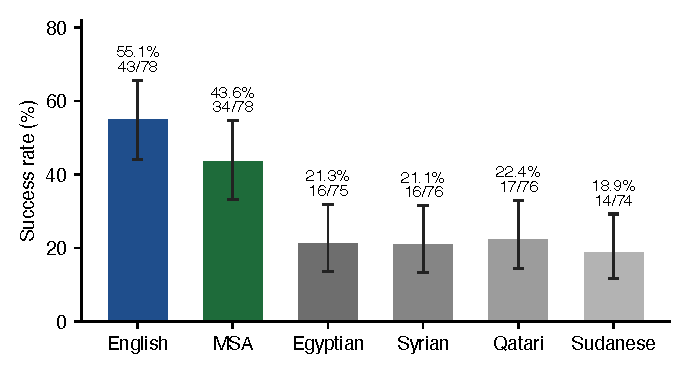
\includegraphics[width=0.62\linewidth]{figures/res_six_language.pdf}
    \caption{Success rate of GPT-5.4 on the same tasks in six languages, with
    95\% Wilson intervals. Each bar's denominator is the number of tasks with a
    genuine verdict in that language.}
    \label{fig:six}
\end{figure}

\paragraph{The gap is real and ordered.}
Figure~\ref{fig:six} and Table~\ref{tab:six} give the main result. English
succeeds on \rateen\% of tasks, MSA on \ratemsa\%, and the four dialects on
between \dialectmin\% and \dialectmax\%. The three tiers are well separated.
On the \npairenmsa{} paired tasks, English beats MSA on \foenmsa{} tasks and
MSA beats English on \soenmsa{} (paired gap \gapenmsa{} points, McNemar
$p=\penmsa$). The drop from MSA to each dialect is larger than the drop from
English to MSA: between \gapmsaqa{} and \gapmsasd{} points, each with
$p<0.001$ (Table~\ref{tab:pairwise}). The dialects are close to one another and
far from MSA: a model that handles MSA is not thereby handling the Arabic that
people actually speak.

\begin{table}[t]
\centering
\small
\begin{tabular}{lrrrr}
\toprule
Language & Valid runs & Pass & Pass rate & 95\% CI \\
\midrule
English & 78 & 43 & 55.1\% & [44.1, 65.7] \\
MSA & 78 & 34 & 43.6\% & [33.1, 54.6] \\
Egyptian & 75 & 16 & 21.3\% & [13.6, 31.9] \\
Syrian & 76 & 16 & 21.1\% & [13.4, 31.5] \\
Qatari & 76 & 17 & 22.4\% & [14.5, 32.9] \\
Sudanese & 74 & 14 & 18.9\% & [11.6, 29.3] \\
\bottomrule
\end{tabular}

\caption{GPT-5.4 success rate by language on the audited borrowed tasks.
Runs with an evaluation error are excluded from the denominator.}
\label{tab:six}
\end{table}

\begin{table}[t]
\centering
\small
\begin{tabular}{llrrrrrr}
\toprule
First & Second & $n$ & Both pass & First only & Second only & Gap (pts) & McNemar $p$ \\
\midrule
English & MSA & 78 & 32 & 11 & 2 & +11.5 & 0.022 \\
MSA & Egyptian & 75 & 13 & 21 & 3 & +24.0 & 0.000 \\
MSA & Syrian & 76 & 14 & 20 & 2 & +23.7 & 0.000 \\
MSA & Qatari & 76 & 14 & 20 & 3 & +22.4 & 0.000 \\
MSA & Sudanese & 74 & 12 & 21 & 2 & +25.7 & 0.000 \\
English & Egyptian & 75 & 15 & 28 & 1 & +36.0 & 0.000 \\
English & Syrian & 76 & 16 & 27 & 0 & +35.5 & 0.000 \\
English & Qatari & 76 & 15 & 28 & 2 & +34.2 & 0.000 \\
English & Sudanese & 74 & 12 & 30 & 2 & +37.8 & 0.000 \\
\bottomrule
\end{tabular}

\caption{Paired comparisons on tasks with a genuine verdict in both languages.
``First only'' counts tasks the first language passed and the second failed.
The McNemar test uses the two discordant counts.}
\label{tab:pairwise}
\end{table}

\paragraph{The ordering holds in every family.}
Figure~\ref{fig:family} splits the result by family. Desktop tasks
(LibreOffice, GNOME, Chrome; $n=\ntasksdesktop$) and terminal tasks
($n=\ntasksterminal$) both show the same English $>$ MSA $>$ dialect order.
The audited web set here is only \ntasksweb{} tasks; the web result comes from
the multi-model experiment below.

\begin{figure}[t]
    \centering
    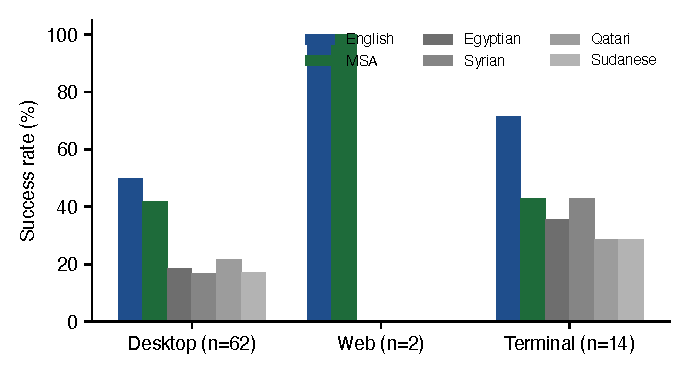
\includegraphics[width=0.62\linewidth]{figures/res_family.pdf}
    \caption{Success rate by family and language for GPT-5.4.}
    \label{fig:family}
\end{figure}

\paragraph{Per-task view.}
Figure~\ref{fig:grid} shows every task as a row and every language as a
column. Of the \ccN{} tasks with a verdict in all six languages,
\ccAllFail{} fail everywhere and \ccAllPass{} pass everywhere; the language
gap lives in the middle. The most common single pattern after all-fail is
``English and MSA pass, all four dialects fail'' (\ccEnMsaOnly{} tasks),
followed by ``English only'' (\ccEnOnly{} tasks). When MSA passes, the
majority of dialects fail on \ccMsaPassDialFail{} tasks and pass on
\ccMsaPassDialPass{}.

\begin{figure}[t]
    \centering
    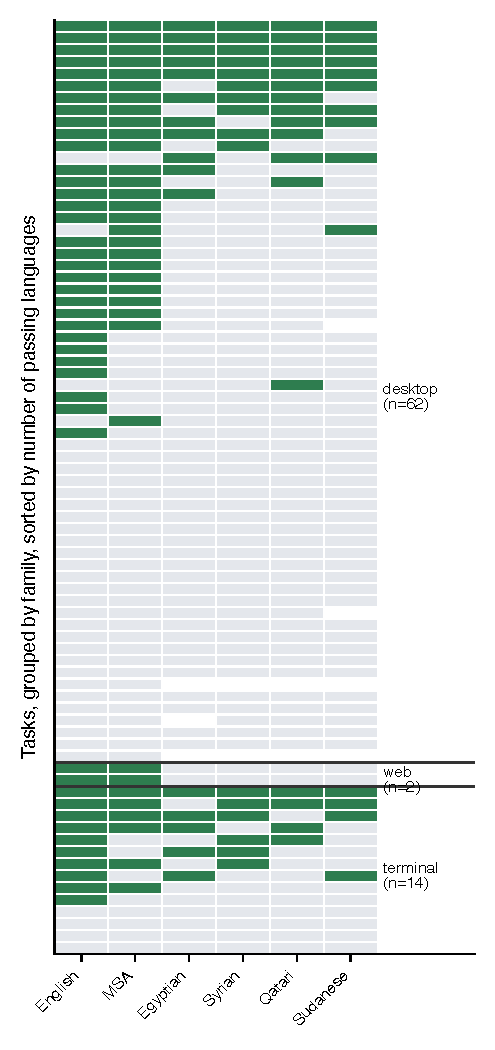
\includegraphics[width=0.5\linewidth]{figures/res_task_grid.pdf}
    \caption{Outcome of every audited task (rows) in every language
    (columns); green is a pass. Rows are grouped by family and sorted by the
    number of languages that pass.}
    \label{fig:grid}
\end{figure}

\paragraph{How runs end.}
Figure~\ref{fig:endings} shows how the failed runs across all six languages
ended. \failDone\% ended with the agent declaring the task done when it was
not, \failSteps\% ran out of steps, and \failGaveUp\% ended with the agent
giving up. The agent's own confidence is therefore not a useful signal: most
failures are runs the agent believed it had completed. Median steps per run
were \medstepsen{} in English and \medstepsmsa{} in MSA; the dialect arms
were shorter (\medstepssy{}--\medstepseg{} steps), consistent with giving up
or declaring done earlier rather than running out of budget.

\begin{figure}[t]
    \centering
    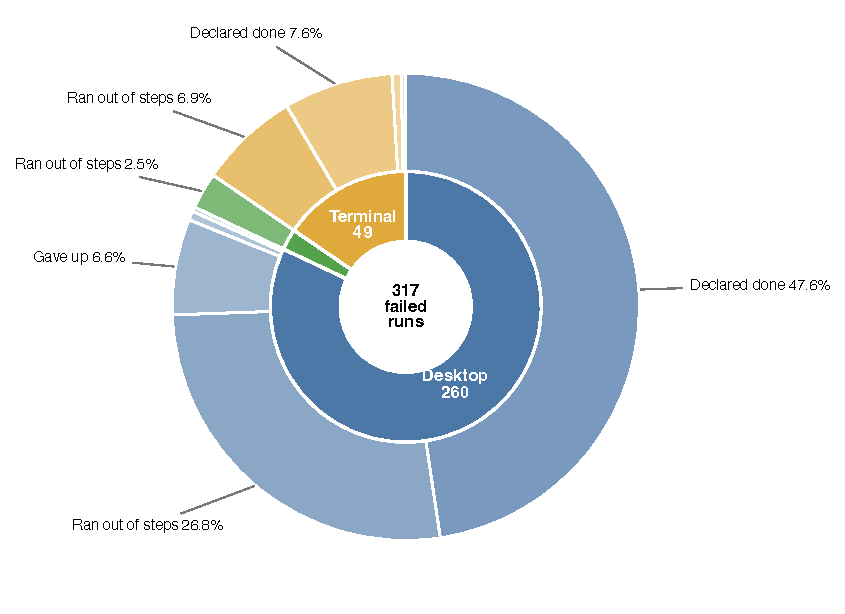
\includegraphics[width=0.55\linewidth]{figures/res_fail_endings.pdf}
    \caption{How failed runs ended, by family (inner ring) and stop reason
    (outer ring), over all six languages.}
    \label{fig:endings}
\end{figure}

\subsection{Four models, English and MSA}
\label{sec:multimodel}

\todo{The four-model experiment on the full 191-task roster (GPT-5.4, Gemini
3.7 Flash, Claude Sonnet 5, Claude Opus 4.8) is running at the time of
writing. This subsection will report: the main model $\times$ family $\times$
language table with paired gaps and McNemar $p$; whether the gap is present
for every model and whether the model ordering is the same in both languages;
the web family split by native-Arabic sites vs browser-translated sites; the
provenance split (human-translated vs model-drafted Arabic arms); and steps
and tokens per arm.}

\paragraph{Comparison with the original benchmarks.}
\todo{Table: our English success rate per model on borrowed tasks beside the
rate the benchmark's own published runs report on the same tasks (from their
released per-task results), noting where the same model was not run upstream
and which model was the closest published one.} Agreement here is a validity
check on the harness rather than a result about language.
